\documentclass[12pt]{extarticle}
\usepackage[utf8]{inputenc}
\usepackage{graphicx}
\usepackage{fancyvrb}
\usepackage{minted}
\usepackage{enumitem}
\usepackage[margin=1.2in]{geometry}
\usepackage{hyperref}
\VerbatimFootnotes

\interfootnotelinepenalty=10000

\title{Rescaling of Timely Dataflow}
\author{Lorenzo Selvatici}
\date{Aug 2019}

\begin{document}

\maketitle

\section{Introduction}

This document summarizes the work done to support dynamic rescaling of timely dataflow\footnote{https://github.com/LorenzSelv/timely-dataflow/tree/rescaling-p2p}.

In a nutshell, timely runs distributed dataflow computation in a cluster. The shape of the cluster is fixed
when first initializing the computation: how many timely processes (likely spread across several machines) and how many worker threads per timely process.
With this project, we allow the addition of new worker processes to the cluster.

In long running jobs with unpredictable workloads, it is likely that the initial configuration will not be the ideal one.
As such, there is the need to scale-out by adding more workers (and scale-in, by removing worker processes).

\section{Timely Model}

* each worker has a copy of the entire dataflow
* async
* progress tracking

\section{Rescaling the computation}

We now go into details of how the rescaling is actually implemented.
Firstly, a high-level overview of the key points that need to be dealt with is given.
Secondly, we present the design options for the initialization of the progress tracking state for the new worker.
Lastly, we describe the integration with Megaphone.

\subsection{Communication Infrastructure}

Rescaling the computation is possible only when running in cluster mode: multiple timely processes, each wrapping several worker
threads, have established connections to each other and exchange both data and progress updates.

In this setting, "adding more workers" means adding another timely process with the same number of worker threads
of every other timely process in the cluster.

Communication among workers happens in two instances:
\begin{itemize}
    \item \verb|exchange| operator
    \item progress updates broadcast
\end{itemize}

In both cases, communication is enabled by \textit{allocating a channel} which contains an endpoint to every other worker
for both sending and receiving (\verb|Pusher| and \verb|Puller| traits, respectively).

Channel allocations happen while building the dataflow within the \verb|worker::dataflow| function call.

If a new worker process joins the cluster, we need to \textit{back-fill} these previously allocated channels.
We do this by storing a closure for each past allocation, so that when the new worker initiates the connection
we can invoke these closures which add the supplied pushers to the list of pushers forming the channel.

Each channel is associated with a specific data type.
Thus, we cannot simply store a map of \verb|(channel id => channel handle)|, as collections can be generic but also need to be homogeneous.
One might work around this by using trait objects, but then the channel would be associated with the trait object itself rather than the concrete
type.

Moreover, fast-forwarding a bit, having a closure turned out to be very handy when implementing the bootstrap protocol to initialize the new worker
progress tracker: when adding the new pusher to the list, we also push a \textit{bootstrap message} that informs the new worker about the next
progress-update sequence number it will receive from that direct connection.


\vspace{3mm}
\noindent
When running in cluster mode, each worker process spawns an extra-thread that will accept incoming connections from workers joining the cluster.
Upon accepting the connection, the thread will spawn a pair of \verb|send| and \verb|recv| network threads, perform some bookkeeping and
finally inform the worker threads about the new timely process that is trying to join the cluster.
This is achieved by sending a \verb|RescaleMessage| on a shared \verb|mpsc| channel.

Worker threads need to explicitly check for rescale messages via the \verb|worker::rescale| function call.
This is done in the very beginning of the \verb|worker::step| function.

With the exception of the \textit{bootstrap} protocol that we will talk about in a later section,
this is all from the perspective of worker processes already in the cluster.

\subsection{New Worker Initialization}

Initialization of the new worker boils down to two things:
\begin{itemize}
    \item building the dataflow (possibly more than one)
    \item initializing the progress tracker
\end{itemize}

We will now talk about them in detail.

\subsubsection{Building the dataflow}
Since the program we use to run the new process is the same to the one of other processes,
the construction of the dataflow comes for free.
The single and very important difference is how we handle \textit{capabilities}.
In particular, generic operators such as \verb|source| and \verb|unary_frontier| supply
a capability to the user-provided constructor, which can use it request notifications
or store it to retain the ability of producing output at a later time.

Clearly, as the new worker can join at any time in the computation, we must not supply
capabilities for timestamps (epochs) that have been closed already as that would allow
the worker to produce output ``in the past''.

Ideally, one would like to have a capability consistent with the frontier
of that operator at the time of joining the cluster: if the new worker joins when
an operator happens to be at some timestamp \verb|t|, it would be fine to provide
a capability for such timestamp to that operator.

% TODO: maybe move to the limitations section

Unfortunately, there are some complications in trying to do this:
\begin{itemize}
    \item As already mentioned, capabilities are passed to the constructor
        of the generic operators while building the dataflow. However, at least
        with the current implementation of the bootstrap protocol, we need to build
        the dataflow \textit{before} actually performing the protocol. But then
        we do not know the operator frontier and thus also the right capability to supply when building the dataflow.

    \item If we do supply a capability for a certain timestamp \verb|t|, we need to ensure
        that no other worker will ever consider that timestamp ``closed'' before the new
        worker discard the capability for that timestamp (e.g. by dropping or downgrading it).

\end{itemize}

For the first item, the issue could be worked-around by sending a map to the new
worker which, for each operator, specifies the frontier of that operator.
Then, while building the dataflow, the new worker would look up in the map the frontiers
and supply appropriate capabilities.

An alternative solution, and the one currently implemented, is to \textit{not} supply capabilities at all to the new worker.
This approach does bring some limitations:
\begin{itemize}
    \item Operators can produce output only in response to some input (which comes with the associated capability for that timestamp).
        As such, \verb|source| operators are useless for new workers: they do not hold any capability and cannot produce any output.
    \item Operators cannot request notifications for future times unless they use capabilities that came with input data.
\end{itemize}

There is an asymmetry between workers which hold capabilities (initial workers present in the cluster)
and are capable of injecting new data in the dataflow (via the \verb|source| operators) and workers
that do not hold capabilities as they joined the cluster at a later time. So, while we can add worker
at runtime, there are some ``special workers''.
Looking from a fault-tolerant perspective, where we would like to allow arbitrary worker to crash without
compromising the execution, making this a potential showstopper.

\vspace{3mm}
For the second item, the bootstrap worker (see later section about the bootstrapping protocol)
should emit a \verb|(t, +1)|\footnote{it should actually be \verb|num_worker_threads| instead of \verb|+1|, as every new worker thread should get a capability}
pointstamp (progress update), to ensure that the timestamp \verb|t| will not be closed
until the corresponding \verb|(t, -1)| pointstamp is emitted.
Such \verb|(t, -1)| will be emitted by the new worker upon downgrading the capability.

\subsubsection{Initializing the Progress Tracker}
The progress tracking protocol is arguably the most important component at the core of timely computational model.
As such we need to ensure that new workers have an up-to-date and correct view of the progress state.

When building the dataflow, each operator is supplied by default with capabilities for timestamp \verb|0| (or the default analogous for different
timestamp types). Some operators do not require capabilities and simply discard them. Other operators use them to request notification,
produce output, etc.
These operations on capabilities are associated with the emission of progress updates, made of a pair \verb|(pointstamp, delta)|.
These progress updates are broadcasted by every worker to all other workers via the established TCP connections between pair of processes.

There are two alternatives to initialize the progress state of the new worker:
\begin{itemize}
    \item Reconstruct a consistent view by all the frontiers of the operator, which have changed over time as a consequence of progress updates
    \item Record and accumulate every progress update that has been sent so that we can apply them again
\end{itemize}

We implemented the second option, as it is easier to reason about and hard to get wrong. Also,
as progress updates tend to cancel each other out (\verb|+1| and \verb|-1| pairs), we \textit{expect}
such accumulation to remain fairly small, no matter how long the computation has been run for.
We should add proper instrumentation to the code to verify this claim.

In the next two sections we present the two alternatives for implementing the above idea:
\verb|pubsub|-based approach and \verb|peer-to-peer|-based approach, both of them
have been implemented to some extent, but \verb|peer-to-peer| turned out to be a better option.

\subsection{Pub-Sub Approach}

One possible design would be to swap the all-to-all communication pattern for progress updates
with an external \verb|pubsub| system. Such system would have established connection to all workers.
Each worker would send its progress updates that will be broadcasted on its behalf. Each worker
then reads progress updates from every other worker.

Progress updates from each worker could be appended to a queue and when every other worker currently
in the cluster has read the progress updates up to a certain point, updates before that point
can be safely compacted (most term would cancel out).

When a new worker joins the cluster, it would ``subscribe'' to every other worker's queue,
initialize its progress tracking state using the compacted updates and finally start reading
new updates from the append-only queue of updates.

A possible implementation of such queue mechanism has been implemented\footnote{https://github.com/LorenzSelv/pubsub}.

\subsubsection{Discussion}

While this sounds like a clean and simple idea, there are a few complications:
\begin{itemize}
    \item To perform updates compaction, the \verb|pubsub| system needs to be aware of timestamp
        data types in the dataflow. Since these timestamps depend on the dataflow that has been constructed,
        the \verb|pubsub| system needs to build the same dataflow, unless we implement some weird export
        mechanism. Moreover, the \verb|pubsub| system needs to use timely data types, which would require
        a circular dependency between the two otherwise-unrelated crates.

    \item More on a philosophical note, adding this external system, which also represents a single point of
        failure, goes a bit against the peer-to-peer spirit of timely.

\end{itemize}

From performances point of view, there would be definitely some overhead associated with the \verb|pubsub|
system itself. Among other things, now there are two hop that a message needs to go through before reaching
its destination. On the other hand, one could easily optimize the amount of progress messages sent around:
you could have a single subscriber per process, so that the same progress messages are not duplicated
because of multiple internal worker threads\footnote{in the current implementation, each progress updates
is sent to every worker thread, thus there are duplicate messages between pair of processes}. This might also solve the communication volume bottleneck
that some experiments show to prevent timely from scaling-out after a certain limit%
\footnote{mostly referring to the results in the Noria paper, but we should perform some proper experiments to investigate this further}.


\subsection{Peer-to-Peer Approach}

An alternative design would be to have the new worker initializes its progress tracking state
by selecting some \textit{bootstrap server} and perform some \textit{bootstrap protocol}.

In particular, the bootstrap server is simply another worker that is selected to help the
new worker initializing its progress tracking state.

The rescale message received by the worker thread contains a flag signaling if the worker thread
was selected as the bootstrap server, and in that case it would initiate the bootstrap protocol.

\subsubsection{Bootstrap Protocol}

Before describing the protocol, we presents some changes needed to make it possible.
To begin with, the server side of the protocol is performed in the \verb|Worker::rescale|\footnote{\verb|timely/src/worker.rs|}
and \verb|TcpAllocator::rescale|\footnote{\verb|communication/src/allocator/zero_copy/allocator.rs|} functions;
the client side of the protocol is performed in the \verb|bootstrap_worker_client|\footnote{\verb|communication/src/rescaling/bootstrap.rs|} function.

Somewhat similarly to the previous approach, each \verb|Progcaster|\footnote{the entity responsible for broadcasting and receiving progress updates
for a specific scope} keeps an accumulation of all progress updates as a \verb|ChangeBatch|.
We define the progress state as this accumulation plus the information about the last sequence number included in the state for each worker.

The bootstrap server, while performing the protocol, does not perform other work. Since it needs to use non-thread-safe data
structures, it was not possible to spawn a separate thread to perform the protocol concurrently.

\begin{figure}[h]
    \centerline{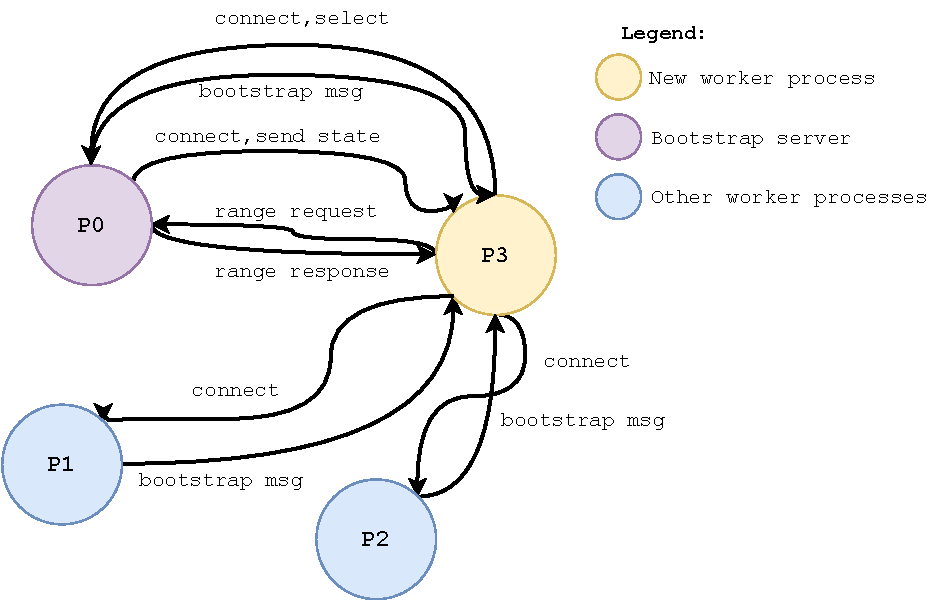
\includegraphics[width=.8\linewidth]{imgs/bootstrapprotocol.pdf}}
    \caption{Bootstrap protocol, timely processes are shown as circles}
    \label{fig:bootstrapprotocol}
\end{figure}

The bootstrap protocol (also depicted in figure \ref{fig:bootstrapprotocol}) consists of the following steps:
We will refer to the new worker joining the cluster as ``bootstrap client''.

\begin{enumerate}
    \item \texttt{Bootstrap client waits for an incoming connection at some arbitrary bootstrap address}.

    \item \texttt{Bootstrap server initiates the connection to that same address.}

    \item \texttt{Bootstrap server sends the progress tracking state to the new worker and start recording following progress updates.}
        The progress tracking state has been defined above. Recording messages simply means appending them to a list (different for each worker)
        so that we can access them at a later time. The lists are cleared at the end of the protocol.

    \item \texttt{Bootstrap server listens for incoming progress-updates-range requests.}

    \item \texttt{Bootstrap client inspects direct TCP connections with other workers, where it will find the bootstrap messages, containing the next progress-update sequence number it will read from that channel.}
        The bootstrap message is the first message that is sent over the newly-established TCP connection.

    \item \texttt{Bootstrap client computes the missing progress updates ranges by comparing the sequence numbers, in the state and the ones in the bootstrap messages.}
        Since the new worker has the guarantee that it will see all progress updates with sequence number greater or equal to the one in the bootstrap
        message, filling the missing gaps between the received progress state and the such sequence numbers guarantees that it will have seen all
        progress updates.

    \item \texttt{Bootstrap client sends progress-updates-range requests to the bootstrap server.}

    \item \texttt{Bootstrap server sends progress-updates-range responses to the bootstrap client.}
        A progress-updates-range request has the format \texttt{(scope\_id, worker\_index, start/end sequence number)}
        which uniquely identifies some updates range. If the bootstrap server cannot fulfill the request
        as it has not seen all requested messages yet, it will pull more progress updates from the channels with the other workers.
        Eventually, all required progress will be received also by the bootstrap server which
        will be then able to fulfill the request.

    \item \texttt{Bootstrap client terminates the bootstrapping protocol by closing the connection.}

\end{enumerate}


\subsection{Megaphone Integration}

After the new worker has joined the cluster and initialized its progress tracking state, it is ready to perform some actual
work. If the dataflow is using plain \verb|exchange| operators, the new worker will start receiving those input data
that hash to its index (modulo the new number of peers).

This ``side effect'' might be acceptable for stateless operator or if the correctness of your computation does \textit{not}
rely on the fact that a worker sees all the input data that hash to the same value.

Most non-trivial operators, however, keep some state used to produce the output when combined to the input data.
A simple WordCount dataflow is a perfect example: to emit the correct count for a word,
a worker should see all occurrences for that word.

As a result, we need to rely on some sort of routing table that gives us such guarantee.
In order to avoid unnecessary overhead for those applications that do not require rescaling or do not need such routing
guarantee, we decided to not provide this feature as part of core timely: we rely on Megaphone instead.

Two main changes where needed to support rescaling operation in Megaphone, we will now describe them.

\subsubsection{Variable number of peers}
After a rescaling operation, the numbers of peers in the cluster has changed. Thus, we must keep a reference
that reflects the current value rather than a simple integer.

\subsubsection{Initializing the new worker Routing State}
When a new worker joins the cluster, it initializes its dataflow and progress tracking state.
However, the bootstrap protocol does not perform any initialization of operators' state, such as the
routing table for Megaphone's stateful operators.

To ensure correctness, we need to make sure that input data are properly routed even by new workers.

As a result, we slightly modified the structure of Megaphone's F operator (the one storing the routing table
and receiving re-configuration commands) by adding a feedback connection with an \verb|exchange| operator
to transfer the routing state from the bootstrap server to the new worker. The routing state is transferred
when the newly introduced \verb|Bootstrap| command is received.
The routing state is made of the currently active routing table plus all future re-configurations.

A rescaling operation consists of the following steps:
\begin{itemize}
    \item The new timely process is spawned, it setups connections and performs the bootstrap protocol. At this
        point, the routing state is not initialized, thus the new worker must not process any input yet.
    \item The controller must send a \verb|Boostrap| command in the control commands stream. The command
        payload specifies the indices of the bootstrap server and of the new worker. It must send a \verb|Bootstrap| command
        for each new worker thread that joined the cluster with the new timely process.
    \item Upon receiving the \verb|Bootstrap| command, the bootstrap server send its routing state to the
        new worker using the feedback-exchange connection we described above.
    \item Upon receiving the routing state, the new worker implants it and can now start to consume input data
        and route them appropriately.
\end{itemize}

For ease when reasoning about the correctness of the protocol that initializes the routing state,
we require that no other control command is issued for the same timestamp of a \verb|Bootstrap| command.

Moreover, we also require that there are no pending configurations changes for which corresponding
control notifications have been already delivered (meaning that the input frontier of the operator reached the
same totally-ordered timestamp of the control command, but the configuration change has not been applied yet).
The reason for this extra constraint is the impossibility to transfer capability associated to the
reconfiguration to the new worker.

We do allow, on the other hand, pending configuration for which notifications have not been delivered yet (``future''
re-configurations). Since we have the guarantee that they have timestamp strictly larger than the bootstrap time,
the new worker can use the capability associated with the receival of the
routing state to setup the corresponding notifications.

\section{Writing Rescalable Timely Programs}

\subsection{Stateless Operators only}

Below is pasted the code for the rescalable \verb|HelloWorld| timely program:

\begin{minted}[linenos, highlightlines={22}, highlightcolor=yellow]{rust}
extern crate timely;

use timely::dataflow::{InputHandle, ProbeHandle};
use timely::dataflow::operators::{Input, Exchange, Inspect, Probe};

fn main() {
    timely::execute_from_args(std::env::args(), |worker| {

        let index = worker.index();
        let mut input = InputHandle::new();
        let mut probe = ProbeHandle::new();

        worker.dataflow(|scope| {
            scope.input_from(&mut input)
                 .exchange(|x| *x)
                 .inspect(move |x| println!("worker {}: seen {}", index, x))
                 .probe_with(&mut probe);
        });

        // if the worker is a new worker joining the cluster,
        // perform the bootstrap protocol.
        if worker.bootstrap() { return; }

        // introduce data and watch!
        for round in 0..10 {
            if index == 0 {
                std::thread::sleep(std::time::Duration::from_secs(1));
                input.send(round);
            }
            input.advance_to(round + 1);
            while probe.less_than(input.time()) {
                worker.step();
            }
        }
    }).unwrap();
}
\end{minted}

The only difference is the call to \verb|worker.bootstrap()| highlighted in the code.
It is a no-op for ``normal'' workers. For new workers joining the cluster, however,
it will perform the bootstrapping protocol to initialize the progress tracking state of the new worker itself.
It is of critical importance that the call is made right after building \textit{all} dataflows,
as it will attempt to initialize the progress state for all dataflows that other workers present
in the cluster have built.

\subsubsection{Sample usage and execution}

Let us compile and run the above program\footnote{source code can be found in at \verb|timely/examples/rescaling/hello.rs|}.
Start a cluster with two timely processes, each with a single worker thread (run in two different terminals):

\vspace{2mm}
\noindent
\verb|$ cargo run --package timely --example rescaling_hello -- -n2 -w1 -p0|

\noindent
\verb|$ cargo run --package timely --example rescaling_hello -- -n2 -w1 -p1|

\vspace{2mm}
Worker 0 will see all even numbers, worker 1 will see all odd numbers.

\noindent
Before the computation has finished, spawn a new timely process, again with a single worker:

\vspace{2mm}
\noindent
\verb|$ cargo run --package timely --example rescaling_hello -- -n2 -w1 -p2 -j 0 --nn 3| 

\vspace{2mm}
\noindent
Note that there are now two extra arguments:
\begin{itemize}
    \item \verb|-j 0| or \verb|--join 0| means that the worker should join the cluster, using worker 0 as the bootstrap server.
        Any worker can be the bootstrap server.
    \item \verb|--nn 3| means that the new number of timely processes in the cluster is now 3.
\end{itemize}

Below we paste the output of a sample execution:

\begin{verbatim}

$ cargo run --package timely --example rescaling_hello -- -n2 -w1 -p0
    Finished dev [unoptimized + debuginfo] target(s) in 0.02s
     Running `target/debug/examples/rescaling_hello -n2 -w1 -p0`
worker 0: seen 0
worker 0: seen 2
worker 0: seen 4
worker 0:       connection from worker 2, bootstrap address is [Some(127.0.0.1:9002)]
bootstrap worker server done!
worker 0: seen 6
worker 0: seen 9
\end{verbatim}


\begin{verbatim}
$ cargo run --package timely --example rescaling_hello -- -n2 -w1 -p1
    Finished dev [unoptimized + debuginfo] target(s) in 0.02s
     Running `target/debug/examples/rescaling_hello -n2 -w1 -p1`
worker 1: seen 1
worker 1: seen 3
worker 1: seen 5
worker 1:       connection from worker 2, bootstrap address is [None]
worker 1: seen 7
\end{verbatim}

\begin{verbatim}
$ cargo run --package timely --example rescaling_hello -- -n2 -w1 -p2 -j0 --nn 3
    Finished dev [unoptimized + debuginfo] target(s) in 0.02s
     Running `target/debug/examples/rescaling_hello -n2 -w1 -p2 -j0 --nn 3`
[bootstrap client] connected to worker 0
workers left: {0, 1}
workers left: {1}
[W2] sent updates range ProgressUpdatesRange { channel_id: 8, worker_index: 1, start_seqno: 9, end_seqno: 10 }
[W2] got updates range response
[W2] applied updates range response
done bootstrapping a worker
worker 2: seen 8
\end{verbatim}

Ignoring some debug output, we see that after worker 2 has joined the cluster, it receives the input integer 8,
as \verb|8 mod 3 = 2|. Same reasoning for worker 0 (and worker 1), it was previously seeing only even numbers
(\verb|X mod 2 = 0|), but after the rescaling operation it receives 6 and 9 as they both result in 0 after the \verb|mod 3|
operation (where \verb|3| is the new number of peers in the cluster).

\subsection{Stateful operators}

Below is a simple \verb|WordCount| example, where we use Megaphone's \verb|stateful_state_machine|
interface to guarantee correctness of emitted word counts (some parts are omitted for brevity):

\begin{minted}[linenos]{rust}
fn main() {
    timely::execute_from_args(std::env::args(), |worker| {
        let mut lines_in = InputHandle::new();
        let mut control_in = InputHandle::new();
        let widx = worker.index();

        worker.dataflow::<usize, _, _>(|scope| {
            let control = control_in.to_stream(scope).broadcast();

            let words_in =
                lines_in
                    .to_stream(scope)
                    .flat_map(|text: String|
                        text.split_whitespace()
                            .map(move |word| (word.to_owned(), 1))
                            .collect::<Vec<_>>()
                    );

            words_in
                // the routing table of an arbitrary worker should route properly
                .exchange(|(word, _)| calculate_hash(word))
                .stateful_state_machine(|key: &String, val, agg: &mut u64| {
                    *agg += val;
                    (false, Some((key.clone(), *agg)))
                }, |key| calculate_hash(key), &control)
                .inspect(move |x| println!("[W{}] stateful seen: {:?}", widx, x))
        });

        if worker.bootstrap() { return; }
        if worker.index() == 0 { /* send lines and reconfiguration commands */ }
    }).unwrap()
}
\end{minted}


Differently from before, when the new worker joins the cluster, it will not receive any input until
some reconfiguration command moves the ownership of some of the bins to it.

A short demo is available at \url{https://www.youtube.com/watch?v=Zsf-eMvHUxU}.



\section{Evaluation}

Changes that might cause an overhead to core timely when running in cluster mode, even if the rescaling feature is not used:

\begin{itemize}
    \item an additional thread is spawned and listens to at some \verb|ip:port| for incoming connection
    \item \verb|allocate| function to allocate a channel now returns a list of pushers wrapped in a \verb|Rc<RefCell<..>>| so it can be mutated when rescaling,
              the pointer need to be dereferenced before usage
    \item progress updates are accumulated in a \verb|ChangeBatch| by each progcaster (this is also true for non-cluster mode)
\end{itemize}

Below is a list of experiments that I believe would be useful to perform to assess performances and back-up some claims with data:

\begin{itemize}
    \item steady-state overhead compared to timely master: how the changes listed above affect the performances in practice
    \item plot per-tuple latency versus time (epochs): how adding a new timely process affects latency both during and after the
        rescaling operation has complete
    \item measure the size of the progress state over time (accumulated progress updates), as a function of
        number of workers and workload type (communication-heavy with lots of exchanges versus in-operator heavy computation and minimal communication).
        We believe that the progress state does not grow in steady-state execution for a fixed number of workers and workload type, as most progress updates
        cancel out.
    \item breakdown of timing in the bootstrap protocol
\end{itemize}

\begin{figure}[h]
    \centerline{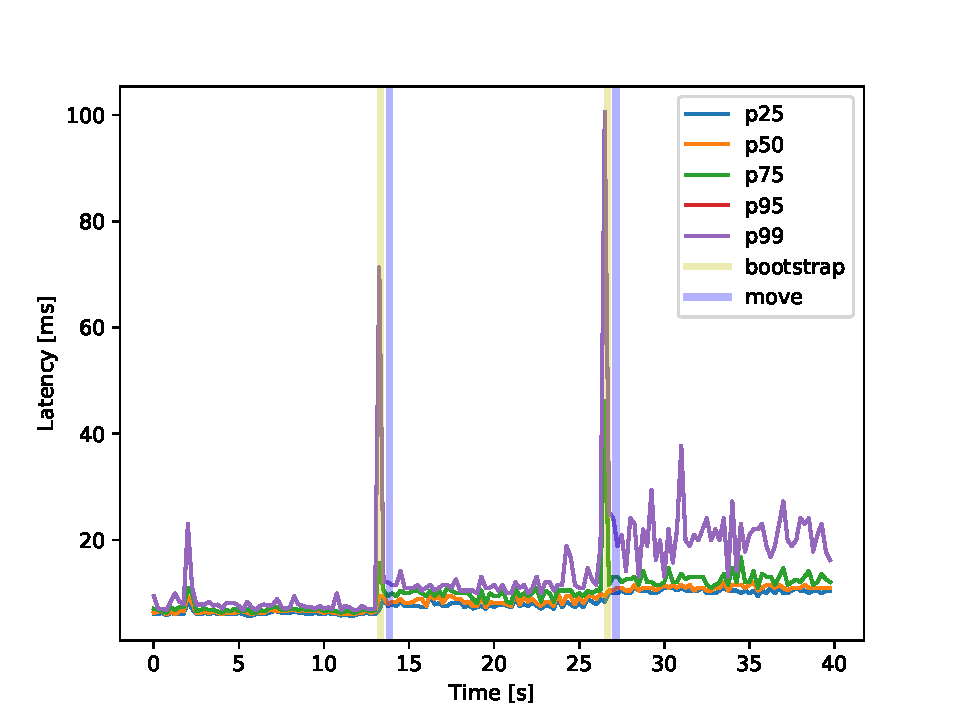
\includegraphics[width=\linewidth]{imgs/latency.pdf}}
    \caption{Latency percentiles for an initial setup of 2x2 workers and 2 rescaling operations, each adding 2 extra workers}
    \label{fig:latency}
\end{figure}

Due to some time constraints, we did not get the chance to run many experiments. In figure \ref{fig:latency} is depicted
a (not very exciting) plot for per-tuple latencies. The experiment setup was as follows:
\begin{itemize}
    \item everything was run on single machine (my personal laptop -- Dell XPS with intel core i7 8th Gen, 16GB RAM)
    \item the initial cluster was made of 2 timely processes, each with 2 worker threads (thus a total of 4 workers)
    \item two rescaling operations were performed, each time adding an additional timely process also with 2 worker threads.
\end{itemize}

The dataflow used is a simple WordCount\footnote{\verb|https://github.com/LorenzSelv/rescaling-examples/blob/master/src/bin/benchmark.rs|} program, where only a single worker samples lines and injects them into the dataflow at a rate of 100 lines per second each with 100 words in it.
Lines are then distributed in a round-robin fashion among workers. The \verb|flat_map| operator splits lines by
whitespaces and emit pairs \verb|(word, 1)|. The \verb|stateful_state_machine| function provided by Megaphone then aggregates the elements by key and counts the occurences.

\vspace{3mm}

From the plot we see that the latency is pretty much constant in the beginning. In correspondence of the first rescaling operation,
there is a spike in latency: a worker is busy performing the bootstrap protocol and the computation is slowed down.

After the new worker joined the cluster we move the ownership of some bins to the new worker with a Megaphone re-configuration command.
However, the latency does not benefit from this rescaling operation as the latency tends to be higher. Out hypothesis is that
the workers already present in the cluster were not saturated before the rescaling operation and adding more workers simply 
increased the communication costs (exchange data and progress messages) which outweighted the benefit of distributing
the workload more evenly among the workers. The second rescaling operation present a similar behaviour.

A better experiment would present saturation in the beginning and, after the rescaling operation a decrease in latency due to the reduce per-worker-load.

I tried to increase the rate of the input, or the length of the lines, but I decided to stop after freezing my machine twice and having to restart it.

\section{Limitations and Future Work}

* no removal of workers
* no capabilities at all for new workers
* formal verification of the protocol

\end{document}
